\documentclass[12pt]{article}
\usepackage{graphicx} % Required for inserting images
\usepackage{enumitem}
\usepackage{mathtools}
\usepackage{amsmath}
\usepackage{gvv-book}
\usepackage{gvv}

\title{\textbf{5.8.2}}
\author{\textbf{EE25BTECH11004 - Aditya Appana}}
\date{September 27, 2025}

\begin{document}

\maketitle

\section*{Question}
10 students of Class X took part in a Mathematics quiz. If the number of girls is 4
more than the number of boys, find the number of boys and girls who took part in
the quiz.

\section*{Solution}

Let the number of girls in the class be $g$, and the number of boys be $b$. Let the vector representing this data be 
\begin{align}
\vec{x} = \myvec{g\\b}    
\end{align}\\
Since the total number of students in the class is 10, $g+b=10$ which can be expressed as:
\begin{align}
\myvec{1\\1}^T\vec{x} = 10
\end{align}\\
Since there are 4 more girls than boys, $b+4=g$, which can be expressed as:
\begin{align}
\myvec{-1 \\ 1}^T\vec{x} = -4
\end{align}\\
Organising these two equations into the form $\vec{A}\vec{x} = \vec{b}$:
\begin{align}
\myvec{1&1 \\ -1&1} \vec{x} = \myvec{10\\-4}
\end{align}\\
Normalising $\vec{A}$: 
\begin{align}
\sqrt{2} \myvec{\frac{1}{\sqrt{2}} & \frac{1}{\sqrt{2}} \\  \frac{-1}{\sqrt{2}}& \frac{1}{\sqrt{2}}} \vec{x} = \myvec{10\\-4}\\
\end{align}\\
Let \myvec{\frac{1}{\sqrt{2}} & \frac{1}{\sqrt{2}} \\  \frac{-1}{\sqrt{2}}& \frac{1}{\sqrt{2}}} be $\vec{M}$. $\vec{M}$ is orthogonal, therefore $\vec{M^T}\vec{M} = \vec{I}$.\\
Multiplying by $\vec{M^T}$ on both the sides:
\begin{align}
\sqrt{2}\vec{x} = \myvec{\frac{1}{\sqrt{2}} & \frac{-1}{\sqrt{2}} \\  \frac{1}{\sqrt{2}}& \frac{1}{\sqrt{2}}} \myvec{10\\-4}\\
\vec{x} = \frac{1}{\sqrt{2}}\myvec{\frac{1}{\sqrt{2}} & \frac{-1}{\sqrt{2}} \\  \frac{1}{\sqrt{2}}& \frac{1}{\sqrt{2}}} \myvec{10\\-4}
\end{align}\\
Solving we get:\begin{align}
\vec{x} = \myvec{7\\3} \\
g = 7\\
b=3
\end{align}

\begin{figure}[H]
    \centering
    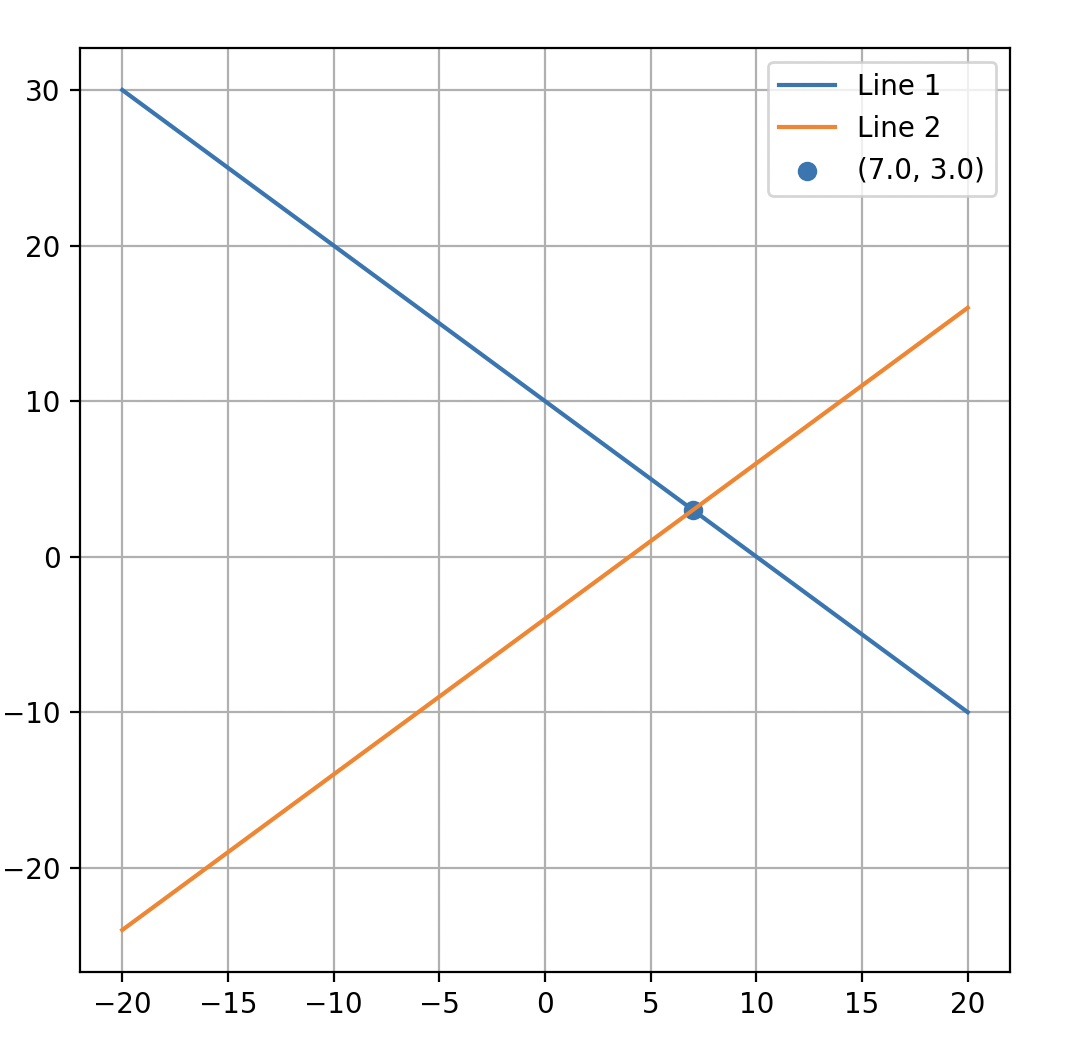
\includegraphics[width=0.6\columnwidth]{Figs/582.png}
    \caption{Plot}
    \label{fig:placeholder}
\end{figure}

\end{document}